\documentclass{standalone}
\usepackage{tikz}
\usetikzlibrary{patterns, positioning}

\begin{document}
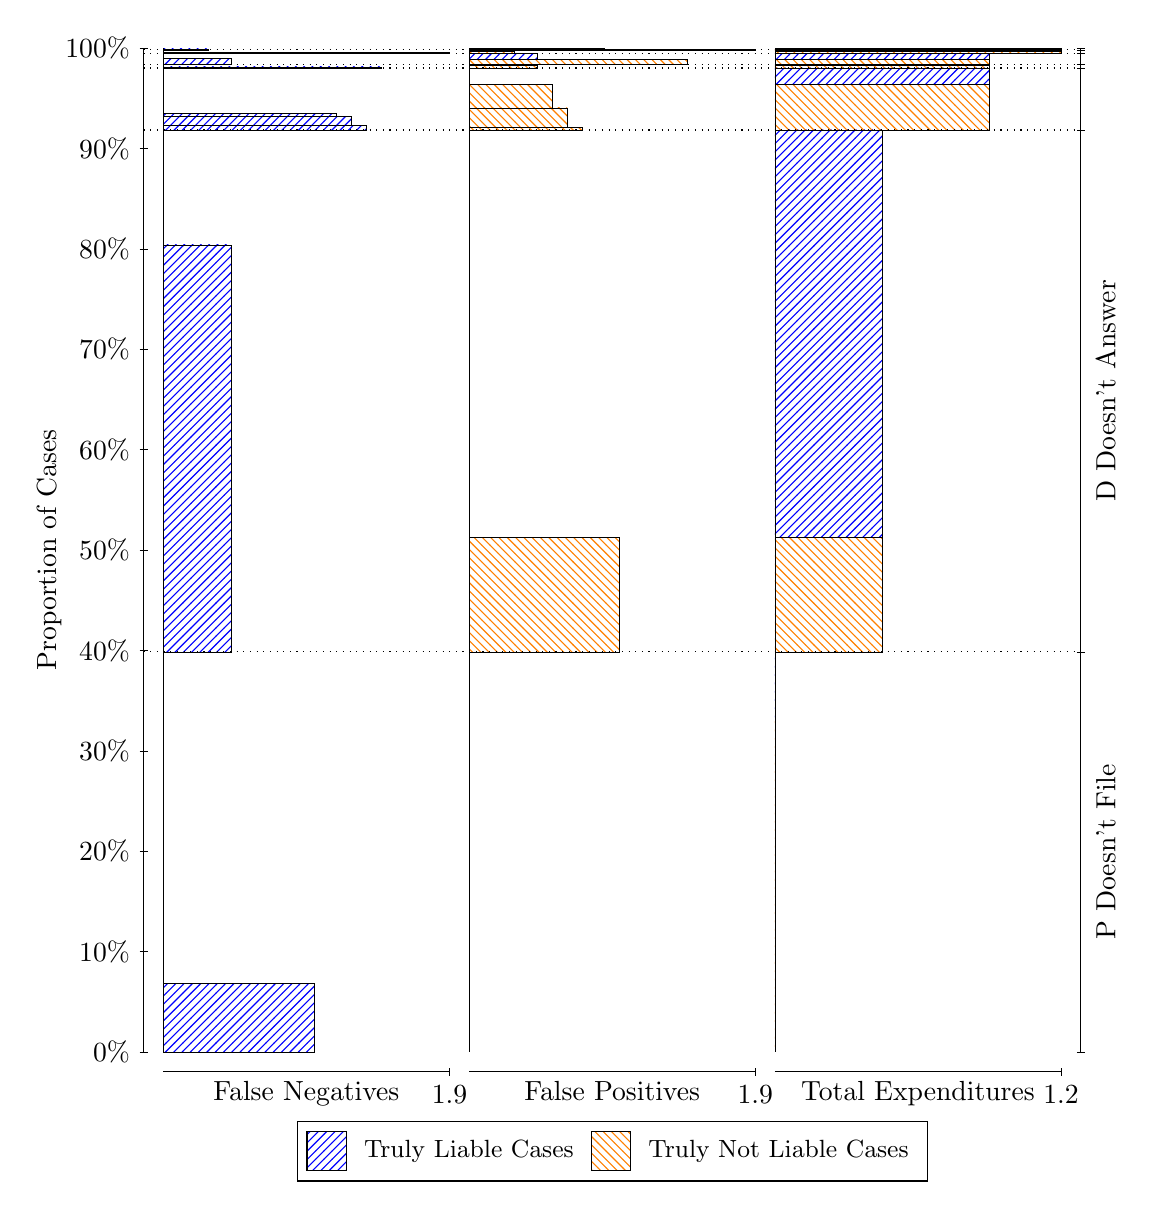
\begin{tikzpicture}
\draw[black, very thin] (1.5,1.75) -- (1.5,14.5);
\node[rotate=90, anchor=center] at (0.3, 8.125) {Proportion of Cases};
\draw[black, very thin] (1.45,1.75) -- (1.55,1.75);
\node[anchor=east] at (1.45, 1.75) {0\%};
\draw[black, very thin] (1.45,3.025) -- (1.55,3.025);
\node[anchor=east] at (1.45, 3.025) {10\%};
\draw[black, very thin] (1.45,4.3) -- (1.55,4.3);
\node[anchor=east] at (1.45, 4.3) {20\%};
\draw[black, very thin] (1.45,5.575) -- (1.55,5.575);
\node[anchor=east] at (1.45, 5.575) {30\%};
\draw[black, very thin] (1.45,6.85) -- (1.55,6.85);
\node[anchor=east] at (1.45, 6.85) {40\%};
\draw[black, very thin] (1.45,8.125) -- (1.55,8.125);
\node[anchor=east] at (1.45, 8.125) {50\%};
\draw[black, very thin] (1.45,9.4) -- (1.55,9.4);
\node[anchor=east] at (1.45, 9.4) {60\%};
\draw[black, very thin] (1.45,10.675) -- (1.55,10.675);
\node[anchor=east] at (1.45, 10.675) {70\%};
\draw[black, very thin] (1.45,11.95) -- (1.55,11.95);
\node[anchor=east] at (1.45, 11.95) {80\%};
\draw[black, very thin] (1.45,13.225) -- (1.55,13.225);
\node[anchor=east] at (1.45, 13.225) {90\%};
\draw[black, very thin] (1.45,14.5) -- (1.55,14.5);
\node[anchor=east] at (1.45, 14.5) {100\%};

\draw[black, very thin] (13.4,1.75) -- (13.4,14.5);
\draw[black, very thin] (13.35,1.75) -- (13.45,1.75);
\node[anchor=west] at (13.35, 1.75) {};
\draw[black, very thin] (13.35,6.8304) -- (13.45,6.8304);
\node[anchor=west] at (13.35, 6.8304) {};
\draw[black, very thin] (13.35,13.459) -- (13.45,13.459);
\node[anchor=west] at (13.35, 13.459) {};
\draw[black, very thin] (13.35,14.247) -- (13.45,14.247);
\node[anchor=west] at (13.35, 14.247) {};
\draw[black, very thin] (13.35,14.291) -- (13.45,14.291);
\node[anchor=west] at (13.35, 14.291) {};
\draw[black, very thin] (13.35,14.433) -- (13.45,14.433);
\node[anchor=west] at (13.35, 14.433) {};
\draw[black, very thin] (13.35,14.476) -- (13.45,14.476);
\node[anchor=west] at (13.35, 14.476) {};
\draw[black, very thin] (13.35,14.5) -- (13.45,14.5);
\node[anchor=west] at (13.35, 14.5) {};

\draw[black, very thin, pattern color=blue, pattern=north east lines] (1.75,1.75) rectangle (3.6623,2.6245);
\draw[black, very thin, pattern color=orange, pattern=north west lines] (1.75,2.6245) rectangle (1.75,6.8304);
\draw[black, very thin, pattern color=blue, pattern=north east lines] (1.75,6.8304) rectangle (2.6105,12.001);
\draw[black, very thin, pattern color=orange, pattern=north west lines] (1.75,12.001) rectangle (1.75,13.459);
\draw[black, very thin, pattern color=blue, pattern=north east lines] (1.75,13.459) rectangle (4.3316,13.521);
\draw[black, very thin, pattern color=blue, pattern=north east lines] (1.75,13.521) rectangle (4.1404,13.631);
\draw[black, very thin, pattern color=blue, pattern=north east lines] (1.75,13.631) rectangle (3.9491,13.669);
\draw[black, very thin, pattern color=orange, pattern=north west lines] (1.75,13.669) rectangle (1.75,14.247);
\draw[black, very thin, pattern color=blue, pattern=north east lines] (1.75,14.247) rectangle (4.5228,14.26);
\draw[black, very thin, pattern color=orange, pattern=north west lines] (1.75,14.26) rectangle (1.75,14.291);
\draw[black, very thin, pattern color=blue, pattern=north east lines] (1.75,14.291) rectangle (2.6105,14.373);
\draw[black, very thin, pattern color=orange, pattern=north west lines] (1.75,14.373) rectangle (1.75,14.433);
\draw[black, very thin, pattern color=blue, pattern=north east lines] (1.75,14.433) rectangle (5.3833,14.445);
\draw[black, very thin, pattern color=orange, pattern=north west lines] (1.75,14.445) rectangle (1.75,14.476);
\draw[black, very thin, pattern color=blue, pattern=north east lines] (1.75,14.476) rectangle (2.3237,14.489);
\draw[black, very thin, pattern color=orange, pattern=north west lines] (1.75,14.489) rectangle (1.75,14.5);
\draw[black, very thin, pattern color=orange, pattern=north west lines] (5.6333,1.75) rectangle (5.6333,5.9559);
\draw[black, very thin, pattern color=blue, pattern=north east lines] (5.6333,5.9559) rectangle (5.6333,6.8304);
\draw[black, very thin, pattern color=orange, pattern=north west lines] (5.6333,6.8304) rectangle (7.5456,8.2884);
\draw[black, very thin, pattern color=blue, pattern=north east lines] (5.6333,8.2884) rectangle (5.6333,13.459);
\draw[black, very thin, pattern color=orange, pattern=north west lines] (5.6333,13.459) rectangle (7.0675,13.497);
\draw[black, very thin, pattern color=orange, pattern=north west lines] (5.6333,13.497) rectangle (6.8763,13.74);
\draw[black, very thin, pattern color=orange, pattern=north west lines] (5.6333,13.74) rectangle (6.6851,14.036);
\draw[black, very thin, pattern color=blue, pattern=north east lines] (5.6333,14.036) rectangle (5.6333,14.247);
\draw[black, very thin, pattern color=orange, pattern=north west lines] (5.6333,14.247) rectangle (6.4939,14.277);
\draw[black, very thin, pattern color=blue, pattern=north east lines] (5.6333,14.277) rectangle (5.6333,14.291);
\draw[black, very thin, pattern color=orange, pattern=north west lines] (5.6333,14.291) rectangle (8.4061,14.352);
\draw[black, very thin, pattern color=blue, pattern=north east lines] (5.6333,14.352) rectangle (6.4939,14.433);
\draw[black, very thin, pattern color=orange, pattern=north west lines] (5.6333,14.433) rectangle (6.207,14.465);
\draw[black, very thin, pattern color=blue, pattern=north east lines] (5.6333,14.465) rectangle (5.6333,14.476);
\draw[black, very thin, pattern color=orange, pattern=north west lines] (5.6333,14.476) rectangle (9.2667,14.487);
\draw[black, very thin, pattern color=blue, pattern=north east lines] (5.6333,14.487) rectangle (7.3544,14.5);
\draw[black, very thin, pattern color=orange, pattern=north west lines] (9.5167,1.75) rectangle (9.5167,5.9559);
\draw[black, very thin, pattern color=blue, pattern=north east lines] (9.5167,5.9559) rectangle (9.5167,6.8304);
\draw[black, very thin, pattern color=orange, pattern=north west lines] (9.5167,6.8304) rectangle (10.879,8.2884);
\draw[black, very thin, pattern color=blue, pattern=north east lines] (9.5167,8.2884) rectangle (10.879,13.459);
\draw[black, very thin, pattern color=orange, pattern=north west lines] (9.5167,13.459) rectangle (12.242,14.036);
\draw[black, very thin, pattern color=blue, pattern=north east lines] (9.5167,14.036) rectangle (12.242,14.247);
\draw[black, very thin, pattern color=orange, pattern=north west lines] (9.5167,14.247) rectangle (12.242,14.277);
\draw[black, very thin, pattern color=blue, pattern=north east lines] (9.5167,14.277) rectangle (12.242,14.291);
\draw[black, very thin, pattern color=orange, pattern=north west lines] (9.5167,14.291) rectangle (12.242,14.352);
\draw[black, very thin, pattern color=blue, pattern=north east lines] (9.5167,14.352) rectangle (12.242,14.433);
\draw[black, very thin, pattern color=orange, pattern=north west lines] (9.5167,14.433) rectangle (13.15,14.465);
\draw[black, very thin, pattern color=blue, pattern=north east lines] (9.5167,14.465) rectangle (13.15,14.476);
\draw[black, very thin, pattern color=orange, pattern=north west lines] (9.5167,14.476) rectangle (13.15,14.487);
\draw[black, very thin, pattern color=blue, pattern=north east lines] (9.5167,14.487) rectangle (13.15,14.5);
\draw[black, dotted] (1.5,6.8304) -- (13.4,6.8304);
\draw[black, dotted] (1.5,13.459) -- (13.4,13.459);
\draw[black, dotted] (1.5,14.247) -- (13.4,14.247);
\draw[black, dotted] (1.5,14.291) -- (13.4,14.291);
\draw[black, dotted] (1.5,14.433) -- (13.4,14.433);
\draw[black, dotted] (1.5,14.476) -- (13.4,14.476);
\draw[black, very thin] (1.75,1.5) -- (5.3833,1.5);
\node[anchor=north] at (3.5667, 1.5) {False Negatives};
\draw[black, very thin] (5.3833,1.45) -- (5.3833,1.55);
\node[anchor=north] at (5.3833, 1.45) {1.9};

\draw[black, very thin] (5.6333,1.5) -- (9.2667,1.5);
\node[anchor=north] at (7.45, 1.5) {False Positives};
\draw[black, very thin] (9.2667,1.45) -- (9.2667,1.55);
\node[anchor=north] at (9.2667, 1.45) {1.9};

\draw[black, very thin] (9.5167,1.5) -- (13.15,1.5);
\node[anchor=north] at (11.333, 1.5) {Total Expenditures};
\draw[black, very thin] (13.15,1.45) -- (13.15,1.55);
\node[anchor=north] at (13.15, 1.45) {1.2};

\node[black, centered, rotate=90] at (13.72, 4.2902) {P Doesn't File};
\node[black, centered, rotate=90] at (13.72, 10.144) {D Doesn't Answer};






\draw (7.449999999999999,1.5) node[draw=none] (baseCoordinate) {};
\begin{scope}[align=center]
        \matrix[scale=0.5, draw=black, below=0.5cm of baseCoordinate, nodes={draw}, column sep=0.1cm]{
            \node[rectangle, draw, minimum width=0.5cm, minimum height=0.5cm, pattern=north east lines, pattern color=blue] {}; &
            \node[draw=none, font=\small] (B) {Truly Liable Cases}; &
            \node[rectangle, draw, minimum width=0.5cm, minimum height=0.5cm, pattern=north west lines, pattern color=orange] {}; &
            \node[draw=none, font=\small] (B) {Truly Not Liable Cases}; \\
            };
\end{scope}

\end{tikzpicture}
\end{document}